\documentclass{../../oss-classkick-exam}
\renewcommand{\arraystretch}{1.2}

\begin{document}
\genheader

\gentitle{20}{CIRCUIT ANALYSIS, PART 1}

\genmultidirections

\gengravity

\raggedcolumns
\begin{multicols}{2}
  \begin{questions}
    \question Five resistors are made of the same material. Which of the
    following has the highest resistance?
    \begin{choices}
      \choice
      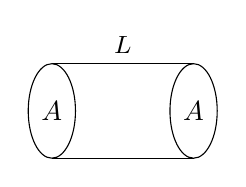
\begin{tikzpicture}[scale=.6]
        \draw ellipse(.5 and 1) node{$A$};
        \draw(3,0) ellipse (.5 and 1) node{$A$};
        \draw(0,1)--(3,1) node[midway,above]{\small$L$};
        \draw(0,-1)--(3,-1);
      \end{tikzpicture}

      \choice
      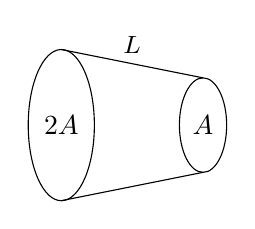
\begin{tikzpicture}[scale=.6]
        \draw ellipse(.7 and 1.6) node{$2A$};
        \draw(3,0) ellipse (.5 and 1) node{$A$};
        \draw(0,1.6)--(3,1) node[midway,above]{\small$L$};
        \draw(0,-1.6)--(3,-1);
      \end{tikzpicture}

      \choice
      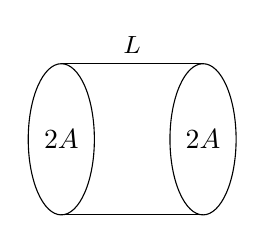
\begin{tikzpicture}[scale=.6]
        \draw ellipse(.7 and 1.6) node{$2A$};
        \draw(3,0) ellipse (.7 and 1.6) node{$2A$};
        \draw(0,1.6)--(3,1.6) node[midway,above]{\small$L$};
        \draw(0,-1.6)--(3,-1.6);
      \end{tikzpicture}

      \choice
      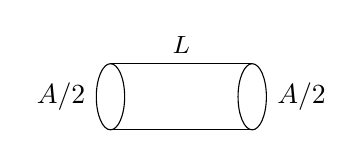
\begin{tikzpicture}[scale=.6]
        \draw ellipse(.3 and .7) node[left]{$A/2\;\;$};
        \draw(3,0) ellipse (.3 and .7) node[right]{$\;\;A/2$};
        \draw(0,.7)--(3,.7) node[midway,above]{\small$L$};
        \draw(0,-.7)--(3,-.7);
      \end{tikzpicture}

      \choice
      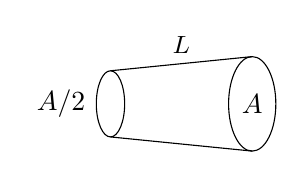
\begin{tikzpicture}[scale=.6]
        \draw ellipse(.3 and .7) node[left]{$A/2\;\;$};
        \draw(3,0) ellipse (.5 and 1) node{$A$};
        \draw(0,.7)--(3,1) node[midway,above]{\small$L$};
        \draw(0,-.7)--(3,-1);
      \end{tikzpicture}
    \end{choices}
    \vspace{.7in}
    
    \uplevel{
      \cpic{.46}{add-resistor}
    }
    \vspace{-.2in}
    \question In the circuit shown, what effect would adding another resistor in
    parallel with the resistor labeled $R$ have?
    \begin{choices}
      \choice The reading on the voltmeter would increase.
      \choice The reading on the ammeter would increase.
      \choice The reading on the voltmeter would decrease.
      \choice The reading on the ammeter would decrease.
      \choice The reading on the ammeter would not change.
    \end{choices}
    \vspace{.7in}
    
    \question The current flowing in a wire as a function of time is given by
    the equation $I=4t^3$. The charge that passes through the wire from
    \SI0{\second} to \SI2{\second} is
    \begin{choices}
      \choice\SI2\coulomb
      \choice\SI4\coulomb
      \choice\SI8\coulomb
      \choice\SI{16}\coulomb
      \choice\SI{24}\coulomb
    \end{choices}
    
%    \question Which of the following statements best summarizes a series circuit
%    with three different resistances?
%    \begin{choices}
%      \choice In all parts of the circuit, the resistances are different, the
%      voltage drops are the same, and the current is different.
%      \choice In all parts of the circuit, the resistances are the same, the
%      voltage drops are the same, and the current is different.
%      \choice In all parts of the circuit, the resistances are different, the
%      voltage drops are different, and the current is the same.
%      \choice In all parts of the circuit, the resistances are different, the
%      voltage drops are the same, and the current is the same.
%      \choice In all parts of the circuit, the resistances are the same, the
%      voltage drops are the same, and the current is the same.
%    \end{choices}
    \uplevel{
      \cpic{.35}{3batteries}
%      \centering
%      \begin{tikzpicture}[yscale=1.5,xscale=1.2]
%        \draw(5,2)--(5,1) to[R,*-](3,1) to[battery,-*](0,1)--(0,2);
%        \draw(5,1)--(5,0)--(3,0) to[battery](0,0)--(0,1);
%        \draw(5,2)--(3,2) to[battery=\mbox{\SI6\volt}](0,2);
%      \end{tikzpicture}
    }
    \question There are three batteries in the circuit shown above. There may
    be other resistances not shown on the diagram. The potential difference
    between points $a$ and $b$ is
    \begin{choices}
      \choice\SI{3}\volt
      \choice\SI{6}\volt
      \choice\SI{9}\volt
      \choice\SI{12}\volt
      \choice\SI{18}\volt
    \end{choices}
    \columnbreak

    \uplevel{
      \textbf{Questions \ref{adjust1}--\ref{adjust2}} An adjustable resistor is
      connected to a battery of emf ε in a simple circuit. A graph of power
      vs.\ current in the battery is shown in the figure.
      \cpic{.45}{adjustable}
    }
    \question The emf $\mathcal E$ of the battery is most nearly
    \label{adjust1}
    \begin{choices}
      \choice 5 V
      \choice 10 V
      \choice 20 V
      \choice 40 V
      \choice 60 V
    \end{choices}
    
    \question What is the resistance of the adjustable resistor when the power
    in the circuit is 10 watts?
    \label{adjust2}
    \begin{choices}
      \choice\SI{1.25}\ohm
      \choice\SI{1.5}\ohm
      \choice\SI{2.5}\ohm
      \choice\SI{5.0}\ohm
      \choice\SI{0}\ohm
    \end{choices}    
    
%    \uplevel{
%      \textbf{Questions \ref{series1}--\ref{series2}}
%      \cpic{.45}{r-in-series}
%    }
%
%    \question Which is the correct ranking of the currents for the resistors?
%    \label{series1}
%    \begin{choices}
%      \choice$I_A=I_B=I_C$
%      \choice$I_A>I_B>I_C$
%      \choice$I_C>I_A=I_B$
%      \choice$I_C>I_B>I_A$
%      \choice$I_C<I_B<I_A$
%    \end{choices}
%
%    \question Which is the correct ranking of the potential differences of the
%    resistors?
%    \label{series2}
%    \begin{choices}
%      \choice $V_A=V_B=V_C$
%      \choice $V_A>V_B>V_C$
%      \choice $V_A=V_B>V_C$
%      \choice $V_C>V_B>V_A$
%      \choice $V_C<V_B<V_A$
%    \end{choices}    
%    \columnbreak
    
    \uplevel{
      \textbf{Questions \ref{bulb1}--\ref{bulb2}}
      Four identical light bulbs are connected to a battery as shown.
      \cpic{.5}{bulbs}
      }
    \question Which bulb will burn the brightest?
    \label{bulb1}
    \begin{choices}
       \choice 1
       \choice 2
       \choice 3
       \choice 4
       \choice All will emit the same brightness.
    \end{choices}
    \vspace{.7in}
    
    \question If bulb 4 is removed, how will the brightness of each of the bulbs
    change, if at all?
    \label{bulb2}
    \begin{choices}
      \choice Bulb 2 will be less bright.
      \choice Bulb 2 will be brighter.
      \choice Bulb 3 will not change its brightness.
      \choice Bulb 1 will not give off light.
      \choice None of the bulbs will change their brightness.
    \end{choices}
%    \vspace{.7in}
%    
%    \uplevel{
%      \textbf{Questions \ref{circ2-1}--\ref{circ2-2}}
%      \begin{center}
%        \begin{tikzpicture}[american voltages,scale=1.3]
%          \draw(0,0) to[battery=$\mathcal E$] (0,2)--(3,2)--(3,1.8);
%          \draw(2,1.8)--(4.4,1.8);
%          \draw(2,0.2)--(4.4,0.2);
%          \draw(2,1.8) to[R=$R_1$] (2,0.2);
%          \draw(3.2,1.8) to[R=$R_2$] (3.2,0.2);
%          \draw(4.4,1.8) to[R=$R_3$] (4.4,0.2);
%          \draw(3,0.2)--(3,0)--(0,0);
%        \end{tikzpicture}
%    
%        \vspace{.1in}$\mathcal E=\SI{12}\volt$, $R_1=\SI{10}\ohm$,\\
%        $R_2=\SI6\ohm$, $R_3=\SI8\ohm$
%      \end{center}
%    }
%
%    \question For the circuit in the diagram, which of the following
%    expressions will describe the amount of current flowing through the
%    resistors?
%    \label{circ2-1}
%    \begin{choices}
%      \choice $I_1=I_2=I_3$
%      \choice $I_3>I_2>I_1$
%      \choice $I_1>I_2<I_3$
%      \choice $I_2>I_1>I_3$
%      \choice $I_1<I_2<I_3$
%    \end{choices}
%    
%    \question For the circuit in the diagram, what is the equivalent resistance?
%    \begin{choices}
%      \choice\SI{.040}\ohm
%      \choice\SI{.40}\ohm
%      \choice\SI{1.}\ohm
%      \choice\SI{2.6}\ohm
%      \choice\SI{24}\ohm
%    \end{choices}
%    
%    \question For the circuit in the diagram, what is the total current?
%    \begin{choices}
%      \choice\SI{.5}\ampere
%      \choice\SI{4.6}\ampere
%      \choice\SI{12}\ampere
%      \choice\SI{30}\ampere
%      \choice\SI{300}\ampere
%    \end{choices}
%    
%    \question For the circuit in the diagram, the third resistor ($R_3$)
%    dissipates how much energy each second?
%    \label{circ2-2}
%    \begin{choices}
%      \choice\SI{12}\watt
%      \choice\SI{14}\watt
%      \choice\SI{46}\watt
%      \choice\SI{212}\watt
%      \choice\SI{300}\watt
%    \end{choices}
  \end{questions}
\end{multicols}
\newpage

\genfreetitle{20}{CIRCUIT ANALYSIS, PART 1}{2}

\genfreedirections

%TAKEN FROM 2015 AP PHYSICS EXAM FREE-RESPONSE QUESTION E&M.2.
\cpic{.25}{find-internal-resistance}

\begin{questions}

  \question A student performs an experiment to determine the emf $\mathcal E$
  and internal resistance $r$ of a given battery. The student connects the
  battery in series to a variable resistance $R$, with a voltmeter across the
  variable resistor, as shown in the figure above, and measures the voltmeter
  reading $V$ as a function of the resistance $R$. The data are
  shown in the table below.
  \begin{center}
    \begin{tabular}{|c|c|c|c|c|}
      \hline
      Trial \# & Resistance (\si\ohm) & Voltage (\si\volt) &
      $1/R$ (\si{\per\ohm}) & $1/V$ (\si{\per\volt}) \\
      \hline
      1 & 0.50 & 5.6 & 2.00 & 0.179 \\ \hline
      2 & 1.0 &  7.4 & 1.00 & 0.135 \\ \hline
      3 & 2.0 &  9.4 & 0.50 & 0.106 \\ \hline
      4 & 3.0 & 10.6 & 0.33 & 0.094 \\ \hline
      5 & 5.0 & 10.9 & 0.20 & 0.092 \\ \hline
      6 & 10 &  11.4 & 0.10 & 0.088 \\ \hline
    \end{tabular}
  \end{center}
  \begin{parts}
    \part
    \label{part1a}
    \begin{subparts}
      \subpart Derive an expression for the measured voltage $V$. Express your
      answer in terms of $R$, $\mathcal E$, $r$, and physical constants, as
      appropriate.

      \subpart Rewrite your expression from part (\ref{part1a})-i to express
      $1/V$ as a function of $1/R$.
    \end{subparts}
    \vspace{1.5in}

    \part On the grid below, plot data points for the graph of $1/V$ as a
    function of $1/R$. Clearly scale and label all axes, including units as
    appropriate. Draw a straight line that best represents the data.
    \label{part1b}
    \begin{center}
      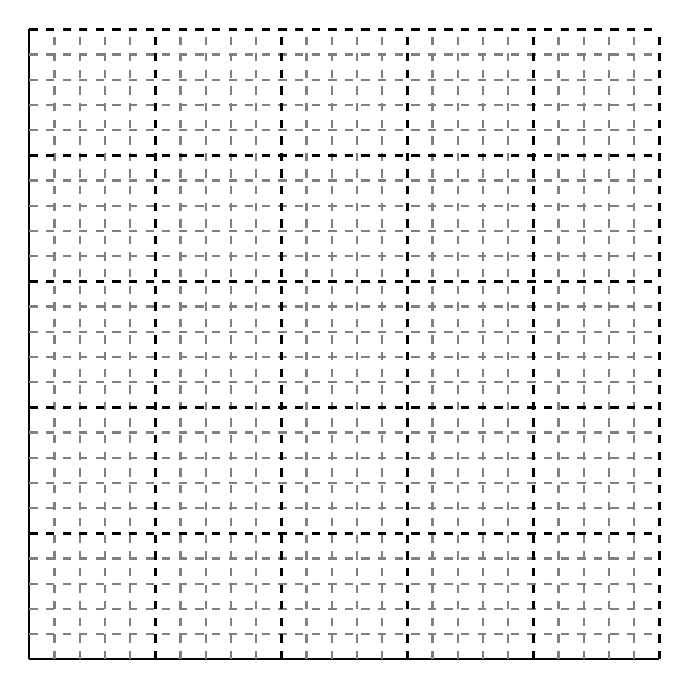
\begin{tikzpicture}[scale=1.6]
        \draw[thick](0,0)--(5,0);
        \draw[thick](0,0)--(0,5);
        \foreach\x in {.2,.4,...,4.8}{
          \draw[thick,dashed,gray](\x,0)--(\x,5);
          \draw[thick,dashed,gray](0,\x)--(5,\x);
        }
        \foreach\x in {1,...,5}{
          \draw[very thick,dashed](\x,0)--(\x,5);
          \draw[very thick,dashed](0,\x)--(5,\x);
        }
      \end{tikzpicture}
    \end{center}

    \part Use the straight line from part (\ref{part1b}) to obtain values for
    the following.
    \begin{subparts}
      \subpart $\mathcal E$
      \subpart $r$
    \end{subparts}
    \newpage
    
    \part Using the results of the experiment, calculate the maximum current
    that the battery can provide.
    \vspace{2in}

    \part A voltmeter is to be used to determine the emf of the battery after
    removing the battery from the circuit. Two voltmeters are available to take
    this measurement---one with low internal resistance and one with high
    internal resistance. Indicate which voltmeter will provide the most
    accurate measurement. Justify your answer.
    
    \vspace{.2in}
    \underline{\hspace{.4in}} The voltmeter with low resistance will provide
    the most accurate measurement.

    \vspace{.2in}
    \underline{\hspace{.4in}} The voltmeter with high resistance will provide
    the most accurate measurement.

    \vspace{.2in}
    \underline{\hspace{.4in}} The two voltmeters will provide equal accuracy.
  \end{parts}
  \newpage

  %TAKEN FROM 2016 AP PHYSICS EXAM FREE-RESPONSE QUESTION E&M.2.
  \uplevel{
    \cpic{.27}{sample}
  }
  \question The circuit shown above consists of a source of variable emf
  $\mathcal E$, an ideal ammeter A, an ideal voltmeter V, a resistor of
  resistance $R$, and a sample of wire with resistance $r$.
  \begin{parts}
    \part How does the current through the wire sample compare with the current
    through the resistor $R$? Justify your answer.
    
    \vspace{.05in}
    \underline{\hspace{.4in}} It is greater through R.
    
    \vspace{.05in}
    \underline{\hspace{.4in}} It is greater through the sample.
    
    \vspace{.05in}
    \underline{\hspace{.4in}} It is the same through both.
    
    \vspace{.05in}
    \underline{\hspace{.4in}} It depends on the resistance of the sample.

    \part How does the potential difference across the wire sample compare with
    the potential difference across the resistor $R$? Justify your answer.
    
    \vspace{.05in}    
    \underline{\hspace{.4in}}It is greater across R.
        
    \vspace{.05in}
    \underline{\hspace{.4in}}It is greater across the sample.
        
    \vspace{.05in}
    \underline{\hspace{.4in}}It is the same across both.
        
    \vspace{.05in}
    \underline{\hspace{.4in}}It depends on the resistance of the sample.

    \uplevel{With the sample of wire in place, the emf of the source is set to
      a given value. The current through and potential difference across the
      resistor $R$ are measured. This is repeated for several values of emf,
      and the data are recorded in the table below.
      \begin{center}
        \begin{tabular}{|c|c|c|p{.5in}|p{.5in}|}
          \hline
          $\mathcal E$ (\si\volt)&  $V_R$ (\si\volt) & $I_R$ (\si\ampere) & &\\
          \hline
          0.250 & 0.179 & 0.162 & & \\ \hline
          0.500 & 0.335 & 0.327 & & \\ \hline
          0.750 & 0.520 & 0.490 & & \\ \hline
          1.000 & 0.670 & 0.687 & & \\ \hline
        \end{tabular}
      \end{center}
    }

    \part Indicate below which quantities should be graphed to yield a straight
    line that could be used to calculate a numerical value for the resistance
    of the wire sample.
    \label{part2c}

    \vspace{.05in}
    Horizontal axis: \underline{\hspace{.5in}}

    \vspace{.05in}
    Vertical axis: \underline{\hspace{.5in}}

    You may use the remaining columns in the table above, as needed, to record
    any quantities that you indicated that are not given.

  
    \part On the grid below, plot the straight line data points from part
    (\ref{part2c}). Clearly scale and label all axes, including units if
    appropriate. Draw a straight line that best represents the data.
    \begin{center}
      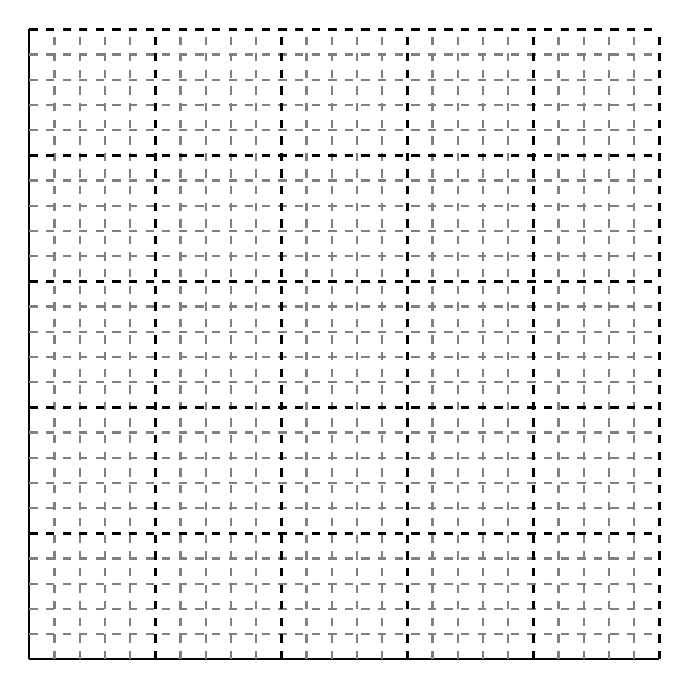
\begin{tikzpicture}[scale=1.6]
        \draw[thick](0,0)--(5,0);
        \draw[thick](0,0)--(0,5);
        \foreach\x in {.2,.4,...,4.8}{
          \draw[thick,dashed,gray](\x,0)--(\x,5);
          \draw[thick,dashed,gray](0,\x)--(5,\x);
        }
        \foreach\x in {1,...,5}{
          \draw[very thick,dashed](\x,0)--(\x,5);
          \draw[very thick,dashed](0,\x)--(5,\x);
        }
      \end{tikzpicture}
    \end{center}
    
    \part Use your straight line to calculate the value of the resistance of
    the wire sample.
    \label{part2e}
    \newpage

    \part The wire sample has a length of \SI{3.00}{\metre} and a radius of
    \SI{1.00e-3}\metre. Calculate the resistivity of the material from which
    the wire sample is made.

    \part
    \begin{subparts}
      \subpart Suppose the ammeter used to collect these data was not ideal.
      Would the actual value of the resistance of the wire sample be greater
      than, less than, or equal to that calculated in part (\ref{part2e})?
      Justify your answer.

      \vspace{.05in}
      \underline{\hspace{.4in}} Greater than\hspace{.5in}
      \underline{\hspace{.4in}} Less than\hspace{.5in}
      \underline{\hspace{.4in}} Equal to
      \vspace{.7in}
      
      \subpart If the ideal voltmeter is replaced by a voltmeter that is not
      ideal and the experiment is repeated, would the readings of the ideal
      ammeter be greater than, less than, or equal to those in the data chart
      before part (\ref{part2c})? Justify your answer.

      \vspace{.05in}
      \underline{\hspace{.4in}} Greater than\hspace{.5in}
      \underline{\hspace{.4in}} Less than\hspace{.5in}
      \underline{\hspace{.4in}} Equal to
      \vspace{.7in}
    \end{subparts}
  \end{parts}
\end{questions}
\end{document}
